%!TEX option = -enable-write18

\documentclass[9pt,xcolor={svgnames, x11names}]{beamer}

% the following two commands 'seem' to do the same thing...?
% \usefonttheme[onlymath]{serif}
\usefonttheme{professionalfonts}

% \usepackage{amsmath} % not needed as this is automatically loaded by Beamer

\definecolor{staticsstructurecolor}{rgb}{0.45,0,0}
% \usepackage{hyperref} % hyperref usually loaded last but automatically be Beamer
\hypersetup{
  colorlinks,
  citecolor=red,
  filecolor=orange,
  linkcolor=staticsstructurecolor, % table of contents
  urlcolor=staticsstructurecolor
}
% \usepackage{enumitem} % incompatible with Beamer?
\everymath{\displaystyle}

\usepackage[absolute,overlay]{textpos}
\setlength{\TPHorizModule}{1.0cm}
\setlength{\TPVertModule}{\TPHorizModule}
\textblockorigin{0.0cm}{0.0cm}  %start all at upper left corner


%\usepackage{amssymb}
\usepackage{verbatim} % for latex code in latex doc
% \usepackage{shellesc}

\usepackage{tikz}
\usepackage{pgfmath}
% \usepackage{fp}
\tikzset{every picture/.append style={line cap=round}}
\def\scale{1} % initialisation for pikz
\usetikzlibrary{calc} % only works within a path
% \usetikzlibrary{fpu}
\usetikzlibrary{math} % if then else etc.
\usetikzlibrary{arrows.meta}


\usetheme{Antibes}
\usecolortheme[named=staticsstructurecolor]{structure}
% \setbeamertemplate{items}[triangle]
\setbeamertemplate{blocks}[rounded][shadow=false]
\setbeamertemplate{headline}{\vspace{.1cm}}
\setbeamertemplate{navigation symbols}{} % empty braces suppresses all navigation symbols
\setbeamertemplate{footline}{
  \hfill
  \insertshorttitle
  \quad
  \insertsection
  \quad
  \insertsubsection
  \quad
  \insertframenumber/\inserttotalframenumber
  \quad{ }
  \vspace{0.125cm}
}
\addtobeamertemplate{footline}{\hypersetup{linkcolor=black}}{}
\setbeamertemplate{navigation symbols}{} % empty braces suppresses all navigation symbols
\setbeamercolor{frametitle}{fg=white}


% counter for resuming enumerated list numbers
\newcounter{resumeenumi}
\newcommand{\suspend}{\setcounter{resumeenumi}{\theenumi}}
\newcommand{\resume}{\setcounter{enumi}{\theresumeenumi}}

\newcommand\lb{\linebreak}
\newcommand\pars{\par\smallskip}
\newcommand\parm{\par\medskip}
\newcommand\parb{\par\bigskip}

%left flushed minipage
\newcommand{\minit}[2][0.8]{
	\begin{minipage}[t]{#1\columnwidth}
		\raggedright
		#2
	\end{minipage}
}

%left flushed minipage
\newcommand{\mini}[2][0.8]{
	\begin{minipage}[c]{#1\columnwidth}
		\raggedright
		#2
	\end{minipage}
}



% centered minipage with text \raggedright
%\cmini[width]{content}
\newcommand{\cmini}[2][0.8]{
	\begin{center}
		\begin{minipage}{#1\columnwidth}
			\raggedright
			#2
		\end{minipage}
	\end{center}
}

% get x and y coordinates from a tikz coordinate
%\gettikzxy{A}{\ax}{\ay}
\makeatletter
\providecommand{\gettikzxy}[3]{%
	\tikz@scan@one@point\pgfutil@firstofone#1\relax
	\edef#2{\the\pgf@x}%
	\edef#3{\the\pgf@y}%
}
\makeatother

\definecolor{saitMaroon}{RGB}{172, 31, 45}
\definecolor{mucus}{rgb}{0.55,0.53,0.31} 
\definecolor{myGreen}{RGB}{0,150,0}
\definecolor{saitPurple}{RGB}{112,40,119}
\definecolor{saitDeepBlue}{RGB}{0, 99, 167}
\definecolor{saitBlue}{rgb}{0, 0.59, 0.85}


%  \definecolor{saitRed}{RGB}{224,38,37} 

%  \definecolor{khaki}{RGB}{190, 183, 107}
 %\definecolor{philpotBlue}{RGB}{13,69,120}
% \definecolor{dRed}{rgb}{0.7,0,0}
% \definecolor{blueGrey}{rgb}{0.4,0.48,0.53}
% \definecolor{white}{rgb}{1,1,1}
% \definecolor{dkgreen}{rgb}{0,0.5,0}
% \definecolor{greenyellow}{rgb}{0.9,0.9,0.5}
% \definecolor{flesh}{rgb}{1, 0.95, 0.8}
% \definecolor{wheat}{rgb}{.96, .87, .70}
% \definecolor{oldlace}{rgb}{.992, .96187, .902}
% \definecolor{snow}{rgb}{1, .98, .98}
% \definecolor{ghostwhite}{rgb}{.973, .973, 1}
% \definecolor{cornsilk}{rgb}{1, .973, .863}
% \definecolor{honeydew}{rgb}{.941, 1, .941}
% \definecolor{lavenderdark}{rgb}{.8, .8, .9529411}
% \definecolor{lavender}{rgb}{.902, .902, .980}
% \definecolor{lightblue}{rgb}{.8, .8, .95}
\definecolor{lightgray}{rgb}{.827, .827, .827}
% \definecolor{lightsteelblue}{rgb}{.690, .769, .871}
% \definecolor{lightturquoise}{rgb}{.686, .933, .933}
% \definecolor{darkgreen}{rgb}{.0, .392, .0}
% \definecolor{yellowgreen}{rgb}{.604, .804, .196}
% \definecolor{vlightblue}{rgb}{.88, .85, .95}
% \definecolor{khaki}{rgb}{.741, .718, .42}
% \definecolor{lightkhaki}{rgb}{1, .96, .7}
% \definecolor{almostwhite}{rgb}{1,.95,1}
% \definecolor{facegreen}{rgb}{.45, .5, .2}
% \definecolor{llllBlueGrey}{rgb}{0.8,0.96,1}
% \definecolor{lllBlueGrey}{rgb}{0.69,0.83,0.92}
% \definecolor{llBlueGrey}{rgb}{0.58,0.69,0.76}
% \definecolor{lBlueGrey}{rgb}{0.48,0.58,0.64}
% \definecolor{blueGrey}{rgb}{0.4,0.48,0.53}
% \definecolor{dBlueGrey}{rgb}{0.33,0.4,0.44}
% \definecolor{ddBlueGrey}{rgb}{0.28,0.33,0.37}
% \definecolor{dddBlueGrey}{rgb}{0.23,0.28,0.31}
% \definecolor{almostBlue}{rgb}{0.985,0.985,1}
% \definecolor{almostGreen}{rgb}{0.9,0.97,0.9}

% \definecolor{almostRed}{rgb}{0.95,0.875,0.8}
%  \definecolor{headerGrey}{RGB}{128,128,128}
%  \definecolor{headerGray}{RGB}{128,128,128}
% \definecolor{dHeaderGrey}{RGB}{96,96,96}
% \definecolor{ddHeaderGrey}{RGB}{64,64,64}
% \definecolor{dddHeaderGrey}{RGB}{32,32,32}
% \definecolor{lHeaderGrey}{RGB}{160,160,160}
% \definecolor{llHeaderGrey}{RGB}{192,192,192}
% \definecolor{lllHeaderGrey}{RGB}{224,224,224}
% \definecolor{philpotBlue}{RGB}{13,69,120}
% \definecolor{drabGreen}{RGB}{156,143,87}
% \definecolor{ground}{RGB}{153,153,51}
% \definecolor{gridLight}{rgb}{0.85,0.85,0.85}
% \definecolor{darkGreen}{rgb}{0,0.5,0}

% !TEX root = ../../statikz/statikz.tex

% get x and y coordinates from a tikz coordinate, returned values in points
\makeatletter
\providecommand{\gettikzxy}[3]{%
  \tikz@scan@one@point\pgfutil@firstofone#1\relax
  \edef#2{\the\pgf@x}%
  \edef#3{\the\pgf@y}%
}
\makeatother

%\Member{startpt}{endpt}{outer}{inner}{stroke}{height}{radius}{line width}
\providecommand{\Member}[8]{
  % name the points
  \coordinate(start) at (#1);
  \coordinate(end) at (#2);
  \def\outer{#3}
  \def\inner{#4}
  \def\stroke{#5}
  \def\hi{#6} % cm
  \def\rad{#7} % cm
  \def\line{#8} % mm

  \def\tocm{0.035146}
  % \def\topt{28.45274}

  \coordinate(delta) at ($ (end)-(start) $);
  \gettikzxy{(delta)}{\dx}{\dy}
  \gettikzxy{(start)}{\sx}{\sy}
  \pgfmathparse{veclen(\dx, \dy)}% \pgfmathresult
  \let\length\pgfmathresult

  \pgfmathparse{\dx==0}%
  % \ifnum low-level TeX for integers
  \ifnum\pgfmathresult=1 % \dx == 0
    \pgfmathsetmacro{\rot}{\dy > 0 ? 90 : -90}
  \else
    \pgfmathsetmacro{\rot}{\dx > 0 ? atan(\dy / \dx) : 180 + atan(\dy / \dx)}
  \fi

  % \begin{scope}[scale=\scale]    
  
    \begin{scope}	[rounded corners = \rad cm, transform canvas = { rotate around = {\rot:(\sx,\sy)}}]
      \shadedraw[top color = \outer, bottom color = \outer, middle color = \inner, draw = \stroke, line width = \line mm] ($ (start)+(-0.5*\hi, 0.5*\hi) $) -- ++(\hi cm +\length pt, 0 ) -- ++(0, -\hi) -- ++ (-\hi cm -\length pt, 0) -- cycle;
    \end{scope}
    % \shadedraw[ball color = \outer!50!\inner, draw = \stroke] (start) circle (\hi/8);
    % \shadedraw[ball color = \outer!50!\inner, draw = \stroke] (end) circle (\hi/8);

% \end{scope}


}


%\Rocker[rotate=0]{coordinate}{fill}{draw}{scale}{line width}
\newcommand{\Rocker}[6][0]{
	\def\rotate{#1};
	\def\coord{#2}
	\def\fill{#3}
	\def\draw{#4}
	\def\scale{#5};
	\def\linewidth{#6};
	\def\h{1}
	\def\r{0.3}

	\begin{scope}[scale=\scale, rotate=\rotate, rounded corners = 3pt]

		\filldraw[draw=\draw, fill=\fill, line width = \linewidth mm] ($(\coord) + (0,-\h)$)arc(-90:-57.54:\h) -- ++(105:0.95394)arc(15:165:\r) -- ++(-105:0.95394)arc(-122.458:-90:\h);

		\shadedraw[ball color=\fill, \draw, line width = 0.75*\linewidth mm] (\coord) circle (1.5mm);
	\end{scope}
}



%\Rone[rotate=0]{coordinate}{draw}{fill}{scale}{line width}
\newcommand{\RollerOne}[6][0]{
	\def\rotate{#1};
	\def\pin{#2}
	\def\lfill{#3}
	\def\ldraw{#4}
	\def\lscale{#5}
	\def\lwidth{#6}
	\def\h{1}
	\def\r{0.3}

	\begin{scope}[scale=\lscale, rotate=\rotate, line width=\lwidth mm]

		\shadedraw[ball color=\lfill!50, draw=\ldraw] ($ (\pin) + (0,-0.6*\h)$) circle (\h*4 mm);
		\filldraw[rounded corners=2pt, draw=\ldraw, fill=\lfill] ($(\pin) + (-0.52494*\h,-.8*\h)$) -- ++(1.05*\h, 0) -- ++(105:0.9059)arc(15:165:\r) -- cycle;
		\shadedraw[ball color=\lfill, draw=\ldraw, line width=2*\lwidth pt] (\pin) circle (\lscale mm);
		\shadedraw[ball color=\lfill, draw=\ldraw, line width=\lwidth pt] ($ (\pin) + (0,-0.6*\h)$) circle (\h*0.5 mm);



	\end{scope}
}



%\Roller[rotate=0]{coordinate}{draw}{fill}{scale}{line width}
\newcommand{\RollerThree}[6][0]{
	\def\rotate{#1};
	\def\pin{#2}
	\def\lfill{#3}
	\def\ldraw{#4}
	\def\lscale{#5};
	\def\lwidth{#6};
	\def\h{1}
	\def\r{0.3}
	\def\rr{0.15}
	\begin{scope}[scale=\lscale, rotate=\rotate, myshade/.style={outer color = \lfill!70!\ldraw, inner color=\lfill!25!white, draw=\ldraw!90!black, line width=\lwidth mm}]
		
		\shadedraw[myshade] ($(\pin) + (0,-\h+\rr)$) circle (\rr);
		\filldraw[\ldraw!50!black]($(\pin) + (0,-\h+\rr)$) circle (0.5mm);

		\shadedraw[myshade] ($(\pin) + (-0.325,-\h+\rr)$) circle (\rr);
		\filldraw[\ldraw!50!black]($(\pin) + (-0.325,-\h+\rr)$) circle (0.5mm);

		\shadedraw[myshade] ($(\pin) + (0.325,-\h+\rr)$) circle (\rr);
		\filldraw[\ldraw!50!black]($(\pin) + (0.325,-\h+\rr)$) circle (0.5mm);

		\filldraw[rounded corners= \lscale pt, draw=\ldraw, fill=\lfill, line width=\lwidth mm] ($(\pin) + (-0.52494*\h,-.8*\h)$) -- ++(1.05*\h, 0) -- ++(105:0.9059)arc(15:165:\r) -- cycle;

		\shadedraw[ball color=\lfill, \ldraw, line width=\lwidth mm] (\pin) circle (1.5mm);
		\filldraw[rounded corners=\lscale pt, draw=\ldraw, fill=\lfill, line width=\lwidth mm] ($ (\pin) - (0.55*\h,0.825*\h) $) rectangle +(1.1*\h,0.2*\h);
	\end{scope}
}




\providecommand{\RollerOnly}[6][0]{
	\def\rotate{#1};
	\def\pin{#2}
	\def\lfill{#3}
	\def\ldraw{#4}
	\def\lScale{#5};
	\def\lwidth{#6};
	\def\h{1}
	\def\r{0.3}
	\def\rr{0.2}
	\begin{scope}[scale=\lScale]
		\begin{scope}[roller/.style={outer color = \lfill, inner color=\lfill!30!black, draw=\ldraw!50!black, line width=\lwidth mm}]
			\shadedraw[roller] (\pin) circle (\h);
			\shadedraw[ball color=\lfill, line width=2*\lwidth pt] (\pin) circle (1.5mm);
		\end{scope}
	\end{scope}
}

\newcommand{\PinnedConnection}[6][0]{
	\def\lrotate{#1}
	\def\lpin{#2}
	\def\lfill{#3}
	\def\ldraw{#4}
	\def\lscale{#5}
	\def\lwidth{#6}
	\def\h{1}
	\def\r{0.3}
	\begin{scope}[scale=\lscale, rotate=\lrotate]
		\filldraw[draw=\ldraw, fill=\lfill, line width=\lwidth mm] ($(\lpin) + (0.201*\h+1.0353*\r ,-0.75*\h)$) -- ++(105: 0.77646*\h+0.26795*\r) arc (15:165:\r) -- ++(-105:0.77646*\h+0.26795*\r) -- cycle;

		\shadedraw[ball color=\lfill, draw=\ldraw, line width = \lwidth mm] (\lpin) circle (1.5mm);

		\filldraw[rounded corners=\lscale pt, draw=\ldraw, fill=\lfill, line width=\lwidth mm] ($ (\lpin) - (1,1.05) $) rectangle +(2,0.35);
	\end{scope}
}


\newcommand{\EyeConnection}[6][0]{
	\def\lrotate{#1};
	\def\lpin{#2}
	\def\lfill{#3}
	\def\ldraw{#4}
	\def\lscale{#5}
	\def\lwidth{#6}
	\def\h{1}
	\def\r{0.3}
	\begin{scope}[scale=\lscale, rotate=\lrotate]
		\filldraw[draw=\ldraw, fill=\lfill, line width=\lwidth mm] ($(\lpin) + (0.201*\h+1.0353*\r ,-0.75*\h)$) -- ++(105: 0.77646*\h+0.26795*\r) arc (15:165:\r) -- ++(-105:0.77646*\h+0.26795*\r) -- cycle;

		\fill[outer color=\lfill, inner color=black] (\lpin) circle (2.5mm);
		\filldraw[fill=white, draw=\ldraw, line width = \lwidth mm] (\lpin) circle (1.25mm);

		\filldraw[rounded corners=\lscale pt, draw=\ldraw, fill=\lfill, line width=\lwidth mm] ($ (\lpin) - (1,1) $) rectangle +(2,0.25);
	\end{scope}
}


\newcommand{\EyeConnectionB}[6][0]{
	\def\lrotate{#1};
	\def\lpin{#2}
	\def\lfill{#3}
	\def\ldraw{#4}
	\def\lscale{#5}
	\def\lwidth{#6}
	%\def\h{1.5}
	\def\r{0.3}
	\begin{scope}[scale=\lscale, rotate=\lrotate]
		\filldraw[draw=\ldraw, fill=\lfill, line width=\lwidth mm] ($(\lpin) + (-0.7,-1.25)$) arc(180:90:.2) -- ++(0.05,0)arc(-90:0:0.2) -- ++(0.05,0.65)arc(225:-45:0.28284)-- ++(0.05,-.65)arc(180:270:.2)-- ++(0.05,0)arc(90:0:0.2) -- cycle;
		\fill[outer color=\lfill, inner color=black, line width = 0] (\lpin) circle (2.25mm);
		\filldraw[fill=white, draw=\ldraw, line width = \lwidth mm] (\lpin) circle (1.25mm);

		\begin{scope}[even odd rule]
			\fill[\lfill] (\lpin) circle (2.5mm)
			(\lpin) circle (2.125mm);
		\end{scope}

		\filldraw[rounded corners=\lscale pt, draw=\ldraw, fill=\lfill, line width=\lwidth mm] ($ (\lpin) - (1,1.5) $) rectangle +(2,0.25);
	\end{scope}
}



% various hacks to get around (apparent?) Beamer titlepage constraints
\title[\color{black} Statikz\textcolor{Maroon}{2020}]{\Huge Statikz}
\subtitle{} % i.e., a blank line
\institute{\small Source code at: {\footnotesize\url{https://github.com/dmorgorg/nuLaTeX/blob/master/statikz2020/statikz.pdf}}}
\author{} % another blanky
\date{\small Last updated on \today}

\begin{document} %%%%%%%%%%%%%%%%%%%%%%%%%%%%%%%%%%%%%%%%%%%%%%%%%%%%%%%%%%%%%%%%%%%%%%%%%%%%%%%%%%

\begin{frame}[plain]
  \titlepage
\end{frame}

\begin{frame}{Table of Contents}
  \begin{minipage}{0.9\textwidth}
    \tableofcontents
  \end{minipage}
  \vfill
\end{frame}

\section{Tikz Components} %%%%%%%%%%%%%%%%%%%%%%%%%%%%%%%%%% Components %%%%%%%%%%%%%%%%%%%%%%%%%%%%%%%%
\centering

%%%%%%%%%%%%%%%%%%%%%%%%%%%%%%%%%%%%%%%%%%%%%%%%%%%%%%%%%%%%%%%%%%%%%%%%%%%%%%%%%%%%%%%%%%%%%%%%%%%
% Note that use of verbatim within Beamer needs fragile setting for frame
% Also, verbatim environment cannot be inside curly braces, {\begin{verbatim}... blows up?
\begin{frame}[fragile]{Tikz Components :: Member}

  \small
  \begin{verbatim}
     \Member{startpt}{endpt}{outer}{inner}{stroke}{height}{radius}{line width}
   \end{verbatim}
  \parb
 
  % \resizebox{0.25\textwidth}{!}{%
  
\begin{tikzpicture}
    \coordinate (A) at (0,0);
    \coordinate (B) at (3,3);
    \coordinate (C) at (8,0);
    \coordinate (D) at (6,-0.5);
    \coordinate (E) at (2,0.5);
    \Member{A}{B}{SlateGray}{SlateGray!25!white}{black}{0.35}{0.175}{.25}
    \Member{A}{E}{DarkMagenta}{DarkMagenta!25!white}{black}{0.35}{0.175}{.25}
    \Member{E}{B}{DarkRed}{DarkRed!25!white}{black}{0.35}{0.175}{.25}
    \Member{E}{D}{DarkOliveGreen}{DarkOliveGreen!25!white}{black}{0.35}{0.175}{.25}
    \Member{D}{B}{SteelBlue}{SteelBlue!25!white}{black}{0.35}{0.175}{.25}
    \Member{C}{B}{DarkKhaki}{DarkKhaki!25!white}{black}{0.35}{0.175}{.25}
    \Member{D}{C}{Goldenrod}{Goldenrod!25!white}{black}{0.35}{0.175}{.25}
  \end{tikzpicture}
  % }

\end{frame}

%%%%%%%%%%%%%%%%%%%%%%%%%%%%%%%%%%%%%%%%%%%%%%%%%%%%%%%%%%%%%%%%%%%%%%%%%%%%%%%%%%%%%%%%%%%%%%%%%%%

\begin{frame}[fragile]{Tikz Components :: PinnedConnection}

  \small
  \begin{verbatim}
    \PinnedConnection[rotate=0]{coordinate}{fill}{draw}{scale}{line width}

    \tikz{
      \coordinate (A) at (0,0);
      \PinnedConnection{A}{DarkKhaki}{Black}{2}{0.5}
    }
  \end{verbatim}

  \vspace{1cm}

  \tikz{
    \coordinate (A) at (0,0);
    % \PinnedConnection[rotate=0]{coordinate}{fill}{draw}{scale}{line width}
    \PinnedConnection{A}{DarkKhaki}{Black}{2}{0.5}
  }

\end{frame}
%%%%%%%%%%%%%%%%%%%%%%%%%%%%%%%%%%%%%%%%%%%%%%%%%%%%%%%%%%%%%%%%%%%%%%%%%%%%%%%%%%%%%%%%%%%%%%%%%%%

\begin{frame}[fragile]{Tikz Components :: RollerOne}

  \footnotesize
  \begin{verbatim}
    \RollerOne[rotate=0]{coordinate}{fill}{draw}{scale}{line width}
  \end{verbatim}

  \vspace{1cm}

  \tikz{
    \coordinate (A) at (0,0);
    \RollerOne{A}{DarkKhaki}{Black}{2}{0.5}
  }

\end{frame}
%%%%%%%%%%%%%%%%%%%%%%%%%%%%%%%%%%%%%%%%%%%%%%%%%%%%%%%%%%%%%%%%%%%%%%%%%%%%%%%%%%%%%%%%%%%%%%%%%%%

\begin{frame}[fragile]{Tikz Components :: RollerThree}

  \footnotesize
  \begin{verbatim}
    \RollerThree[rotate=0]{coordinate}{fill}{draw}{scale}{line width}
  \end{verbatim}

  \vspace{1cm}

  \tikz{
    \coordinate (A) at (0,0);
    \RollerThree{A}{DarkKhaki}{Black}{2}{0.5}
  }

\end{frame}
%%%%%%%%%%%%%%%%%%%%%%%%%%%%%%%%%%%%%%%%%%%%%%%%%%%%%%%%%%%%%%%%%%%%%%%%%%%%%%%%%%%%%%%%%%%%%%%%%%%

\begin{frame}[fragile]{Tikz Components :: RollerOnly}

  \footnotesize
  \begin{verbatim}
    \RollerOnly[rotate=0]{coordinate}{fill}{draw}{scale}{line width}
  \end{verbatim}

  \vspace{1cm}

  \tikz{
    \coordinate (A) at (0,0);
    \RollerOnly{A}{DarkKhaki}{Black}{2}{0.5}
  }

\end{frame}
%%%%%%%%%%%%%%%%%%%%%%%%%%%%%%%%%%%%%%%%%%%%%%%%%%%%%%%%%%%%%%%%%%%%%%%%%%%%%%%%%%%%%%%%%%%%%%%%%%%

\begin{frame}[fragile]{Tikz Components :: Rocker}

  \footnotesize
  \begin{verbatim}
    \Rocker[rotate=0]{coordinate}{fill}{draw}{scale}{line width}
  \end{verbatim}

  \vspace{1cm}

  \tikz{
    \coordinate (A) at (0,0);
    % \Rocker[rotate=0]{coordinate}{fill}{draw}{scale}{line width}
    \Rocker{A}{DarkKhaki}{Black}{2}{0.5}
  }

\end{frame}
%%%%%%%%%%%%%%%%%%%%%%%%%%%%%%%%%%%%%%%%%%%%%%%%%%%%%%%%%%%%%%%%%%%%%%%%%%%%%%%%%%%%%%%%%%%%%%%%%%%

\begin{frame}[fragile]{Tikz Components :: EyeConnection}

  \footnotesize
  \begin{verbatim}
    \EyeConnection[rotate=0]{coordinate}{fill}{draw}{scale}{line width}
  \end{verbatim}

  \vspace{1cm}

  \tikz{
    \coordinate (A) at (0,0);
    \EyeConnection{A}{DarkKhaki}{Black}{2}{0.5}
  }

\end{frame}
%%%%%%%%%%%%%%%%%%%%%%%%%%%%%%%%%%%%%%%%%%%%%%%%%%%%%%%%%%%%%%%%%%%%%%%%%%%%%%%%%%%%%%%%%%%%%%%%%%%

\begin{frame}[fragile]{Tikz Components :: EyeConnectionB}

  \small
  \begin{verbatim}
    \EyeConnectionB[rotate=0]{coordinate}{fill}{draw}{scale}{line width}
  \end{verbatim}

  \vspace{1cm}

  \tikz{
    \coordinate (A) at (0,0);
    \EyeConnectionB{A}{DarkKhaki}{Black}{2}{0.5}
  }

\end{frame}

%%%%%%%%%%%%%%%%%%%%%%%%%%%%%%%%%%%%%%%%%%%%%%%%%%%%%%%%%%%%%%%%%%%%%%%%%%%%%%%%%%%%%%%%%%%%%%%%%%%

\section{Qwizm Blanks}
\subsection{GCSE Maths}
\subsection{Math Review}




%%%%%%%%%%%%%%%%%%%%%%%%%%%%%%%%%%%%%%%%%%%%%%%%%%%%%%%%%%%%%%%%%%%%%%%%%%%%%%%%%%%%%%%%%%%%%%%%%%%
\begin{frame}{pikz/01MathReview/math01Qwizm}
    \resizebox{0.75\textwidth}{!}{%
    % !TEX root = ../../statikz2020/statikz2020.tex


\makeatletter
\providecommand{\gettikzxy}[3]{%
	\tikz@scan@one@point\pgfutil@firstofone#1\relax
	\edef#2{\the\pgf@x}%
	\edef#3{\the\pgf@y}%
}
\makeatother


\begin{tikzpicture}[scale=\scale]

	\def\thickness{thick}
	% \def\stroke{black}
	\def\hi{.225}
	\def\radii{.225}
	\def\extend{0.225}

	\def\offset{0.4}

	\coordinate (E) at (0,0);
	\coordinate (F) at (3,0);
	\coordinate (G) at (6,0);
	\coordinate (A) at (9,0);
	\coordinate (B) at (6,2.5);
	\coordinate (C) at (3,3.75);
	\coordinate (D) at (0,5);
	\coordinate (Right) at ($ (A)+(1.5,0)$);
	\coordinate (Bottom) at ($ (A)+(0,-1.5)$);

	\shade[right color = DarkGrey, left color = LightGrey] ($(D)+(-0.66,1)$) rectangle ($(E)+(-2,-1.5)$);
	\draw[thick, black] ($(D)+(-0.66,1)$) -- ($(E)+(-0.66,-1.5)$);

	\PinnedConnection[-90]{D}{DarkGrey}{black}{0.65}{0.25}
	\PinnedConnection[-90]{E}{DarkGrey}{black}{0.65}{0.25}


	\gettikzxy{(A)}{\ax}{\ay}
	\gettikzxy{(B)}{\bx}{\by}
	\gettikzxy{(C)}{\cx}{\cy}
	\gettikzxy{(D)}{\ddx}{\ddy}
	\gettikzxy{(E)}{\ex}{\ey}
	\gettikzxy{(F)}{\fx}{\fy}
	\gettikzxy{(G)}{\gx}{\gy}
	\gettikzxy{(Right)}{\rx}{\ry}
	\gettikzxy{(Bottom)}{\bbx}{\bby}

	\draw ($ (A)+(\offset,0)$) -- (\rx,\ay);
	\draw ($ (B)+(1.25*\offset,0)$) -- (\rx,\by);
	\draw ($ (C)+(2*\offset,0)$) -- (\rx,\cy);
	\draw ($ (D)+(2*\offset,0)$) -- (\rx,\ddy);
	\draw ($ (D)+(0, -\offset)$) -- (\ex,\ey+1.25*\offset cm);
	\draw ($ (E)+(0, -\offset)$) -- (\ex,\bby);
	\draw ($ (F)+(0, -\offset)$) -- (\fx,\bby);
	\draw ($ (G)+(0, -\offset)$) -- (\gx,\bby);
	\draw ($ (A)+(0, -\offset)$) -- (\ax,\bby);

	\Large
	\draw[latex-latex] (\ex,\bby+\offset cm) -- node[fill=white] {$\qquad\quad $}(\fx,\bby+\offset cm);
	\draw[latex-latex] (\fx,\bby+\offset cm) -- node[fill=white] {$\qquad\quad $}(\gx,\bby+\offset cm);
	\draw[latex-latex] (\gx,\bby+\offset cm) -- node[fill=white] {$\qquad\quad $}(\ax,\bby+\offset cm);
	\draw[latex-latex] (\rx-\offset cm,\ay) -- node[fill=white, inner sep=3mm] {$\qquad\quad $}(\rx-\offset cm,\by);
	\draw[latex-latex] (\rx-\offset cm,\by) -- node[fill=white, inner sep=3mm] {$\qquad\quad $}(\rx-\offset cm,\cy);
	\draw[latex-latex] (\rx-\offset cm,\cy) -- node[fill=white, inner sep=3mm] {$\qquad\quad $}(\rx-\offset cm,\ddy);
	

	% \pgfoonew \BC=new rr(B,C,Burlywood1,black, 0.2)
	% \pgfoonew \CD=new rr(C,D,Burlywood1,black, 0.2)
	% \pgfoonew \EF=new rr(E,F,Burlywood1,black, 0.2)
	% \pgfoonew \FG=new rr(G,F,Burlywood1,black, 0.2)
	% \pgfoonew \AG=new rr(A,G,Burlywood1,black, 0.2)
	% \pgfoonew \AB=new rr(A,B,Burlywood1,black, 0.2)
	% \pgfoonew \CE=new rr(C,E,Burlywood1,black, 0.2)
	% \pgfoonew \BF=new rr(B,F,Burlywood1,black, 0.2)
	% \pgfoonew \CF=new rr(C,F,Burlywood1,black, 0.2)
	% \pgfoonew \BG=new rr(B,G,Burlywood1,black, 0.2)

	\Member{B}{C}{DarkKhaki}{DarkKhaki!25}{black}{0.35}{0.175}{.25}
    \Member{C}{D}{DarkKhaki}{DarkKhaki!25}{black}{0.35}{0.175}{.25}
    \Member{E}{F}{DarkKhaki}{DarkKhaki!25}{black}{0.35}{0.175}{.25}
    \Member{F}{G}{DarkKhaki}{DarkKhaki!25}{black}{0.35}{0.175}{.25}
    \Member{A}{G}{DarkKhaki}{DarkKhaki!25}{black}{0.35}{0.175}{.25}
    \Member{A}{B}{DarkKhaki}{DarkKhaki!25}{black}{0.35}{0.175}{.25}
	\Member{C}{E}{DarkKhaki}{DarkKhaki!25}{black}{0.35}{0.175}{.25}
	\Member{B}{F}{DarkKhaki}{DarkKhaki!25}{black}{0.35}{0.175}{.25}
    \Member{C}{F}{DarkKhaki}{DarkKhaki!25}{black}{0.35}{0.175}{.25}
    \Member{B}{G}{DarkKhaki}{DarkKhaki!25}{black}{0.35}{0.175}{.25}

	

	

	\shadedraw[ball color=Burlywood4] (A) circle (2.5pt) node[xshift=2mm, yshift=-3mm] {$A$};
	\shadedraw[ball color=Burlywood4] (B) circle (2.5pt) node[xshift=2.5mm, yshift=3.5mm] {$B$};
	\shadedraw[ball color=Burlywood4] (C) circle (2.5pt) node[xshift=2.5mm, yshift=3.5mm] {$C$};
	\shadedraw[ball color=Burlywood4] (D) circle (2.5pt) node[xshift=2.5mm, yshift=3.5mm] {$D$};
	\shadedraw[ball color=Burlywood4] (E) circle (2.5pt) node[xshift=2mm, yshift=-4mm] {$E$};
	\shadedraw[ball color=Burlywood4] (F) circle (2.5pt) node[xshift=2mm, yshift=-4mm] {$F$};
	\shadedraw[ball color=Burlywood4] (G) circle (2.5pt) node[xshift=2mm, yshift=-4mm] {$G$};



	% \draw[very thin,color=gray] (-0.3,-2.3) grid (2.9,3.3);
	% \draw[->] (-0.2,0) -- (3.2,0) node[right] {$x$};
	% \draw[->] (0,-2.5) -- (0,3.8) node[above] {$y$};
	% \draw[domain=-0.2:2.5, color=red, thick] plot[id=1] function{(7-2*x)/3}
	% node[below] {$2x+3y=7$};
	% \draw[domain=-0.2:0.8, color=blue, thick] plot[id=2] function{6*x-1}
	% node[right] {$6x-y=1$};

\end{tikzpicture}

  }
\end{frame}

%%%%%%%%%%%%%%%%%%%%%%%%%%%%%%%%%%%%%%%%%%%%%%%%%%%%%%%%%%%%%%%%%%%%%%%%%%%%%%%%%%%%%%%%%%%%%%%%%%%
\begin{frame}{pikz/01MathReview/math02Qwizm}
  \resizebox{0.75\textwidth}{!}{%
  % !TEX root = ../../statikz2020/statikz2020.tex


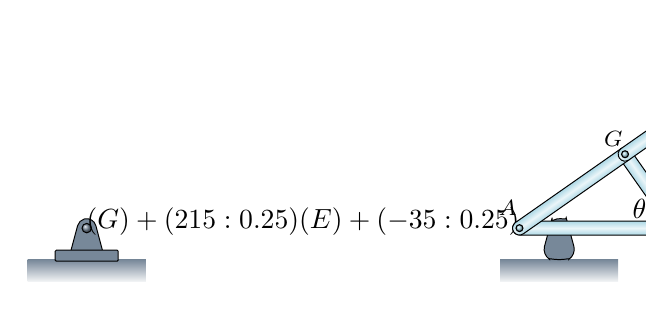
\begin{tikzpicture}

    % \def\offset{0.4}  

	\coordinate (A) at (0,0);
	\coordinate (B) at (2,0);
	\coordinate (C) at (4,0);
    \coordinate (D) at (6,0);
    \coordinate (F) at (3,2.1);
	\coordinate (E) at ($ (D)!0.4468!(F) $);	
    \coordinate (G) at ($ (A)!0.4468!(F) $); 
    
    \gettikzxy{(A)}{\ax}{\ay}
	\gettikzxy{(B)}{\bx}{\by}
	\gettikzxy{(C)}{\cx}{\cy}
	\gettikzxy{(D)}{\dx}{\dy}
	\gettikzxy{(E)}{\ex}{\ey}
	\gettikzxy{(F)}{\fx}{\fy}
    \gettikzxy{(G)}{\gx}{\gy}

	\shade[top color = LightSlateGray, bottom color = LightSlateGray!10] ($(A)+(-0.75,-0.4)$) rectangle +(1.5,-0.275);
    \shade[top color = LightSlateGray, bottom color = LightSlateGray!10] ($(D)+(-0.75,-0.4)$) rectangle +(1.5,-0.275);
    
    
    \Rocker{D}{LightSlateGray}{black}{0.4}{0.125}
    \PinnedConnection{A}{LightSlateGray}{black}{0.4}{0.125}
    
    \draw[thin, black] (\ax, \ay-0.175cm) -- ++(0,-1.125);
    \draw[thin, black] (\bx, \ay-0.175cm) -- ++(0,-1.125);
    \draw[thin, black] (\cx, \ay-0.175cm) -- ++(0,-1.125);
    \draw[thin, black] (\dx, \ay-0.175cm) -- ++(0,-1.125);
    \draw[thin, black] (\fx-0.35cm, \fy) -- (\ax-1cm,\fy);
    \draw[thin, black] (\ax-0.25cm, \ay) -- (\ax-1cm,\ay);

    \draw[Stealth-Stealth] (\ax, \ay-1cm) -- node[fill=white]{\qquad\qquad}(\bx, \by-1cm);
    \draw[Stealth-Stealth] (\bx, \ay-1cm) -- node[fill=white]{\qquad\qquad}(\cx, \by-1cm);
    \draw[Stealth-Stealth] (\cx, \ay-1cm) -- node[fill=white]{\qquad\qquad}(\dx, \by-1cm);
    \draw[Stealth-Stealth] (\ax-0.625cm, \ay) -- node[fill=white, inner sep=2mm]{\qquad\qquad}(\ax-0.625cm, \fy);
    
    % \draw[thin] ($ (G)+(35:0.25) $) -- ++(-55:0.25)--++(215:0.25);
    \draw[thin] ($ (G)+(215:0.25) $) -- ++(305:0.25)--++(35:0.25);
    \draw[thin] ($ (E)+(-35:0.25) $) -- ++(-125:0.25)--++(145:0.25);
    % \draw[thin] ($ (E)+(145:0.25) $) -- ++(235:0.25)--++(325:0.25);

    \node[xshift=-4.75mm,yshift=2.5mm] at (B) {$\theta$};
    \node[xshift=3.5mm, yshift=2.5mm] at (B) {$\phi$};
    	
    \Member{C}{E}{LightBlue}{LightBlue!25}{black}{0.175}{0.0874}{0.125}
    \Member{B}{G}{LightBlue}{LightBlue!25}{black}{0.175}{0.0874}{0.125}
	\Member{A}{B}{LightBlue}{LightBlue!25}{black}{0.175}{0.0874}{0.125}
	\Member{B}{F}{LightBlue}{LightBlue!25}{black}{0.175}{0.0874}{0.125}
	\Member{C}{F}{LightBlue}{LightBlue!25}{black}{0.175}{0.0874}{0.125}
    \Member{C}{D}{LightBlue}{LightBlue!25}{black}{0.175}{0.0874}{0.125}
    \Member{D}{E}{LightBlue}{LightBlue!25}{black}{0.175}{0.0874}{0.125}
    \Member{E}{F}{LightBlue}{LightBlue!25}{black}{0.175}{0.0874}{0.125}
    \Member{A}{G}{LightBlue}{LightBlue!25}{black}{0.175}{0.0874}{0.125}
	\Member{G}{F}{LightBlue}{LightBlue!25}{black}{0.175}{0.0874}{0.125}
	\Member{B}{C}{LightBlue}{LightBlue!25}{black}{0.175}{0.0874}{0.125}
	
    \footnotesize
	\shadedraw[ball color=LightBlue] (A) circle (1.25pt) node[xshift=-1.5mm, yshift=2.5mm] {$A$};
	\shadedraw[ball color=LightBlue] (B) circle (1.25pt) node[xshift=2mm, yshift=-2.5mm] {$B$};
	\shadedraw[ball color=LightBlue] (C) circle (1.25pt) node[xshift=2mm, yshift=-2.5mm] {$C$};
	\shadedraw[ball color=LightBlue] (D) circle (1.25pt) node[xshift=1.5mm, yshift=2.5mm] {$D$};
	\shadedraw[ball color=LightBlue] (E) circle (1.25pt) node[xshift=1.5mm, yshift=2mm] {$E$};
	\shadedraw[ball color=LightBlue] (F) circle (1.25pt) node[yshift=2.5mm] {$F$};
    \shadedraw[ball color=LightBlue] (G) circle (1.25pt) node[xshift=-1.5mm, yshift=2mm] {$G$}; 
    
    

\end{tikzpicture}

}
\end{frame}

%%%%%%%%%%%%%%%%%%%%%%%%%%%%%%%%%%%%%%%%%%%%%%%%%%%%%%%%%%%%%%%%%%%%%%%%%%%%%%%%%%%%%%%%%%%%%%%%%%%
\begin{frame}{pikz/01MathReview/math03Qwizm}
  % !TEX root = ../../statikz2020/statikz2020.tex


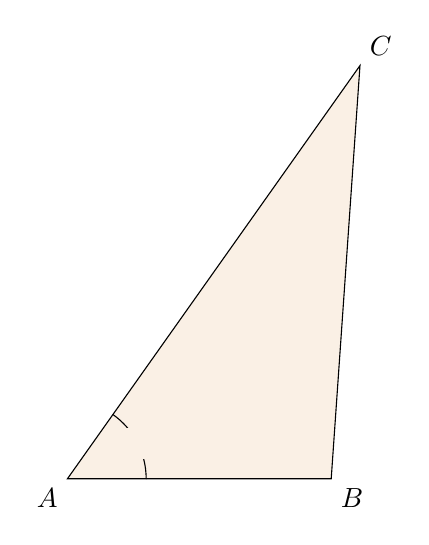
\begin{tikzpicture}[scale=\scale]

	\coordinate (A) at (0,0);
	\coordinate (B) at (3.35,0);
	\coordinate (C) at ($ (A) + (54.7:6.43) $);

	\filldraw[fill=Linen, draw=black] (A) -- (B) -- (C) --  cycle;
	
	\draw[below right] (B) node {$B$};
	\draw[below left] (A) node {$A$};
	\draw[above right] (C) node {$C$};

	\draw (1,0)  arc(0:54.7:1) node[xshift=2mm, fill=Linen, inner sep=2mm] at (24:1.1){$\qquad$};



\end{tikzpicture}

\end{frame}

%%%%%%%%%%%%%%%%%%%%%%%%%%%%%%%%%%%%%%%%%%%%%%%%%%%%%%%%%%%%%%%%%%%%%%%%%%%%%%%%%%%%%%%%%%%%%%%%%%%
\begin{frame}{pikz/01MathReview/math04Qwizm}
  % !TEX root = ../../statikz2020/statikz2020.tex

\resizebox{0.5\textwidth}{!}{%
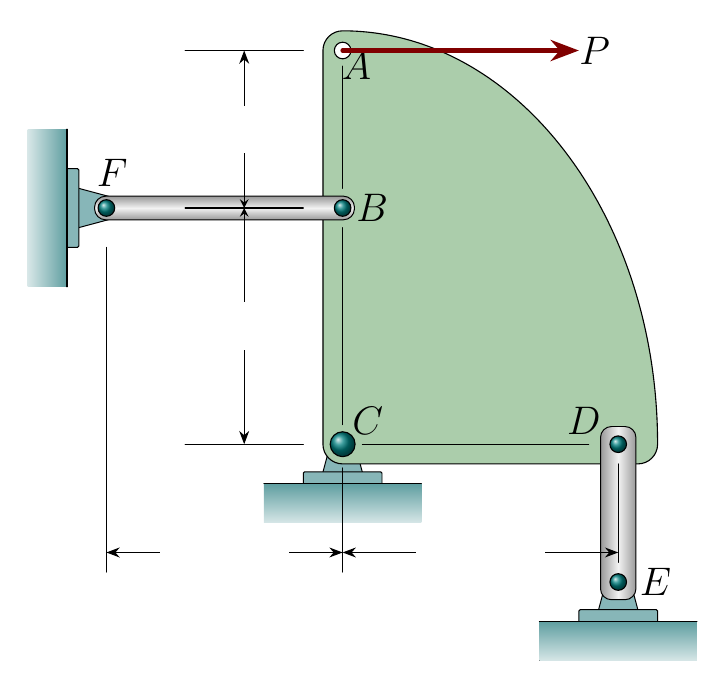
\begin{tikzpicture}

	\coordinate (C) at (0,0);
	\coordinate (B) at (0,3);
	\coordinate (A) at (0,5);
	\coordinate (D) at (3.5,0);
	\coordinate (E) at (3.5,-1.75);
    \coordinate (F) at (-3,3);

    \gettikzxy{(A)}{\ax}{\ay}
    \gettikzxy{(B)}{\bx}{\by}
    \gettikzxy{(C)}{\cx}{\cy}
    \gettikzxy{(D)}{\dx}{\dy}
    \gettikzxy{(E)}{\ex}{\ey}
    \gettikzxy{(F)}{\fx}{\fy}
    
    \PinnedConnection{C}{CadetBlue!75}{Black}{0.5}{0.125};
    \filldraw[fill=DarkSeaGreen!75, draw=black] ($ (A)+(0,0.25)$) arc(90:180:0.25) --($ (C)+(-0.25,0) $)arc(180:270:0.25) -- ($ (D)+(0.25,-0.25)$)arc(270:360:0.25)arc[start angle=0, end angle=90, x radius=4cm, y radius=5.25cm];

    \PinnedConnection[-90]{F}{CadetBlue!75}{Black}{0.5}{0.125};
    
    \PinnedConnection{E}{CadetBlue!75}{Black}{0.5}{0.125};
    \Member{F}{B}{Grey!80!white}{Grey!10}{black}{0.3}{0.14}{0.125};
    \Member{D}{E}{Grey!80!white}{Grey!10}{black}{0.45}{0.14}{0.125};
    
    \filldraw[fill=white, draw=black] (A) circle (3pt) node[xshift=1.75mm, yshift=-2mm]{\Large $A$};
    \shadedraw[ball color=Teal] (B) circle (3pt) node[right, xshift=0.5mm]{\Large $B$};
    \shadedraw[ball color=Teal] (C) circle (4.5pt) node[above right]{\Large $C$};
    \shadedraw[ball color=Teal] (D) circle (3pt) node[above left, xshift=-1mm]{\Large $D$};
    \shadedraw[ball color=Teal] (E) circle (3pt) node[right, xshift=1.5mm]{\Large $E$};
    \shadedraw[ball color=Teal] (F) circle (3pt) node[above, xshift=0.75mm, yshift=1.5mm]{\Large $F$};

    \fill[right color=CadetBlue, left color=CadetBlue!25] (\fx-0.5cm,\fy+1cm) rectangle ++(-0.5,-2);
    \fill[top color=CadetBlue, bottom color=CadetBlue!25] (\cx-1cm,\cy-0.5cm) rectangle ++(2,-0.5);
    \fill[top color=CadetBlue, bottom color=CadetBlue!25] (\ex-1cm,\ey-0.5cm) rectangle ++(2,-0.5);
    \draw (\fx-0.5cm,\fy+1cm) -- ++(0,-2);
    \draw (\cx-1cm,\cy-0.5cm) -- ++(2,0);
    \draw (\ex-1cm,\ey-0.5cm) -- ++(2,0);
    

    \draw ($ (F) + (0,-0.5) $) -- ($ (\fx, \ey+0.125cm)$);
    \draw ($ (D)+(0,-0.25)$) -- ($ (E)+(0,0.25) $);
    \draw ($ (C)+(0,-0.3)$) -- ($ (\cx, \ey+0.125cm) $);
    \draw ($ (A)+(0,-0.2)$) -- ($ (B)+(0,0.25) $);
    \draw ($ (B)+(0,-0.25)$) -- ($ (C)+(0,0.25) $);
    \draw ($ (A)+(-0.5,0)$) -- +(-1.5,0);
    \draw ($ (B)+(-0.5,0)$) -- +(-1.5,0);
    \draw ($ (C)+(-0.5,0)$) -- +(-1.5,0);
    \draw ($ (C)+(0.25,0)$) -- ($(D)+(-0.375,0)$);
    \draw [Stealth-stealth] ($ (A)+(-1.25,0)$) -- node[fill=white, inner sep=3mm]{$\quad$}($ (B)+(-1.25,0)$);
    \draw [stealth-Stealth] ($ (B)+(-1.25,0)$) -- node[fill=white, inner sep=3mm]{$\quad$}($ (C)+(-1.25,0)$);
    \draw [Stealth-Stealth] ($ (\fx, \ey+0.375cm)$) -- node[fill=white]{$\qquad\qquad$}($ (\cx, \ey+0.375cm)$);
    \draw [Stealth-Stealth] ($ (\cx, \ey+0.375cm)$) -- node[fill=white]{$\qquad\qquad$}($ (\ex, \ey+0.375cm)$);

    \draw [-Stealth, ultra thick, Maroon] (A)--+(3,0)node[black, xshift=2mm]{\Large $P$};


   




\end{tikzpicture}
}

\end{frame}

%%%%%%%%%%%%%%%%%%%%%%%%%%%%%%%%%%%%%%%%%%%%%%%%%%%%%%%%%%%%%%%%%%%%%%%%%%%%%%%%%%%%%%%%%%%%%%%%%%%
\begin{frame}{pikz/01MathReview/math05Qwizm}
  % !TEX root = ../../statikz2020/statikz2020.tex

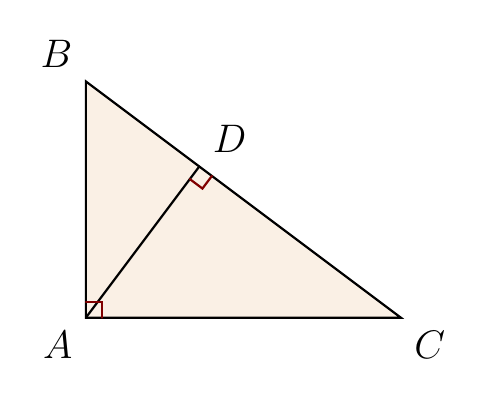
\begin{tikzpicture}

    \Large

	\coordinate (A) at (0,0);
	\coordinate (B) at (0,3);
	\coordinate (C) at (4,0);
	\coordinate (D) at ($(B)!0.36!(C)$);	

    \gettikzxy{(A)}{\ax}{\ay}
    \gettikzxy{(B)}{\bx}{\by}
    \gettikzxy{(C)}{\cx}{\cy}
    \gettikzxy{(D)}{\dx}{\dy}
    
    \filldraw[fill=Linen, thick] (A)--(B)--(C)--cycle; 
    \draw[thick] (A)--(D); 
    \draw[Maroon, thick] (\ax+2mm,\ay)-- ++(0,0.2)-- ++(-0.2,0);
    \draw[Maroon, thick] ($(D)+(-36.9:0.2)$)-- ++(-126.9:0.2)-- ++(143.1:0.2);

    \node[below left] at (A){$A$};
    \node[above left] at (B){$B$};
    \node[below right] at (C){$C$};
    \node[above right] at (D){$D$};

\end{tikzpicture}


\end{frame}

%%%%%%%%%%%%%%%%%%%%%%%%%%%%%%%%%%%%%%%%%%%%%%%%%%%%%%%%%%%%%%%%%%%%%%%%%%%%%%%%%%%%%%%%%%%%%%%%%%%
\begin{frame}{pikz/01MathReview/math06Qwizm}
  % !TEX root = ../../statikz2020/statikz2020.tex

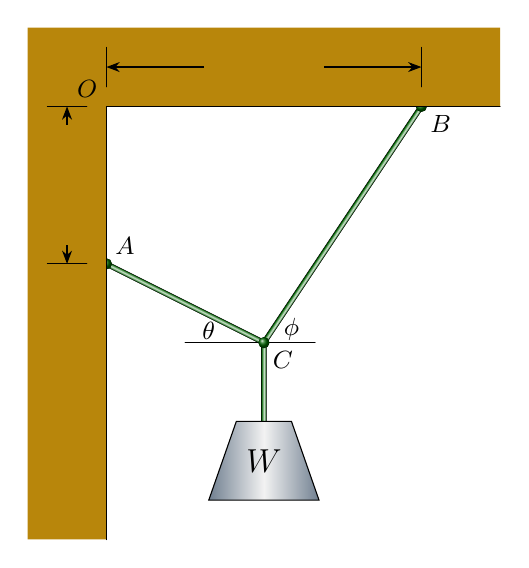
\begin{tikzpicture}   

	\coordinate (O) at (0,0);
	\coordinate (A) at (0,-2);
	\coordinate (B) at (4,0);
	\coordinate (C) at (2,-3);	
	\coordinate (W) at (2,-4);	

    \gettikzxy{(A)}{\ax}{\ay}
    \gettikzxy{(B)}{\bx}{\by}
    \gettikzxy{(C)}{\cx}{\cy}
    \gettikzxy{(O)}{\ox}{\oy}

    \small
    \draw[thin] ($(C)+(-1,0)$)--($(C)+(0.65,0)$);
    \Member{A}{C}{DarkGreen}{DarkGreen!20}{black}{0.0625}{0.014}{0.0625};
    \Member{B}{C}{DarkGreen}{DarkGreen!20}{black}{0.0625}{0.014}{0.0625};
    \Member{C}{W}{DarkGreen}{DarkGreen!20}{black}{0.0625}{0.014}{0.0625};

    \fill[ball color=DarkGreen]  (A)circle(2pt)node[above right]{$A$};
    \fill[ball color=DarkGreen]  (B)circle(2pt)node[below right]{$B$};
    \fill[ball color=DarkGreen]  (C)circle(2pt)node[below right]{$C$};

    \fill[fill=DarkGoldenrod] ($(A)+(0,-3.5)$)--(O)--($(B)+(1,0)$)-- ++(0,1)--(\ox-1cm,\oy+1cm)--(\ox-1cm,\ay-3.5cm)--cycle;
    \draw ($(A)+(0,-3.5)$)--(O)--($(B)+(1,0)$);

    \node[above left] at (O) {$O$};

    \node[xshift=-0.7cm,yshift=1.5mm] at (C) {$\theta$};
    \node[xshift=0.35cm,yshift=1.75mm] at (C) {$\phi$};

    \shade[left color = SlateGray, right color = SlateGray, middle color = Silver!20](\cx+0.35cm,\cy-1cm)-- ++(0.35,-1)-- ++(-1.4,0)-- ++(0.35,1)--cycle;
    \draw (\cx+0.35cm,\cy-1cm)-- ++(0.35,-1)-- ++(-1.4,0)-- ++(0.35,1)--cycle;

    \draw (\ax-2.5mm,\ay)--(\ax-7.5mm,\ay);
    \draw (\ox-2.5mm,\oy)--(\ox-7.5mm,\oy);
    \draw[Stealth-Stealth] (\ax-5mm,\ay)--node[fill=DarkGoldenrod, sloped]{$\qquad\qquad$ }(\ox-5mm,\oy);

    \draw (\ox,\oy+2.5mm)--(\ox,\oy+7.5mm);
    \draw (\bx,\by+2.5mm)--(\bx,\by+7.5mm);
    \draw[Stealth-Stealth] (\ox,\oy+5mm)--node[fill=DarkGoldenrod, sloped]{$\qquad\qquad$}(\bx,\by+5mm);
    
    \node at ($(C)+(0,-1.5)$){\large $W$};

\end{tikzpicture}

\end{frame}


%%%%%%%%%%%%%%%%%%%%%%%%%%%%%%%%%%%%%%%%%%%%%%%%%%%%%%%%%%%%%%%%%%%%%%%%%%%%%%%%%%%%%%%%%%%%%%%%%%%
\section{Math Review}
%%%%%%%%%%%%%%%%%%%%%%%%%%%%%%%%%%%%%%%%%%%%%%%%%%%%%%%%%%%%%%%%%%%%%%%%%%%%%%%%%%%%%%%%%%%%%%%%%%%

% \begin{frame}{pikz/01MathReview/math01}
%   Note: $a, b$ and $c$ are shown after transition.
%   \vspace{1cm}
%   % !TEX root = ../../statikz2020/statikz2020.tex

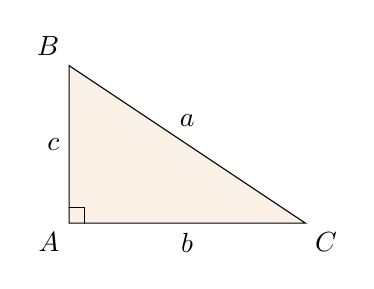
\begin{tikzpicture}[scale=\scale]

	\coordinate (A) at (0,0);
	\coordinate (B) at (0,2);
	\coordinate (C) at (3,0);

	\filldraw[fill=Linen, draw=black] (A) -- (B) -- (C) -- cycle;
	\draw ($ (A)+(0.2,0) $) -- ++(0,0.2) -- ++(-0.2,0);

	\draw[above left] (B) node {$B$};
	\draw[below left] (A) node {$A$};
	\draw[below right] (C) node {$C$};

	\only<2->{
		\node[above, yshift=1mm] at ($ (B)!0.5!(C) $) {$a$};
		\node[left] at ($ (A)!0.5!(B) $) {$c$};
		\node[below] at ($ (A)!0.5!(C) $) {$b$};
	}

\end{tikzpicture}

% \end{frame}

%%%%%%%%%%%%%%%%%%%%%%%%%%%%%%%%%%%%%%%%%%%%%%%%%%%%%%%%%%%%%%%%%%%%%%%%%%%%%%%%%%%%%%%%%%%%%%%%%%%
\begin{frame}{pikz/01MathReview/math01}
  \resizebox{0.75\textwidth}{!}{%
    % !TEX root = ../../statikz2020/statikz2020.tex

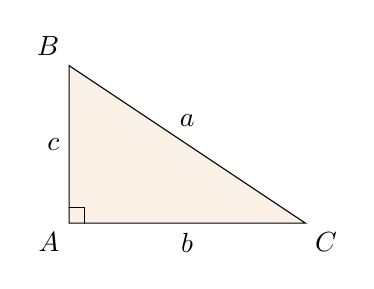
\begin{tikzpicture}[scale=\scale]

	\coordinate (A) at (0,0);
	\coordinate (B) at (0,2);
	\coordinate (C) at (3,0);

	\filldraw[fill=Linen, draw=black] (A) -- (B) -- (C) -- cycle;
	\draw ($ (A)+(0.2,0) $) -- ++(0,0.2) -- ++(-0.2,0);

	\draw[above left] (B) node {$B$};
	\draw[below left] (A) node {$A$};
	\draw[below right] (C) node {$C$};

	\only<2->{
		\node[above, yshift=1mm] at ($ (B)!0.5!(C) $) {$a$};
		\node[left] at ($ (A)!0.5!(B) $) {$c$};
		\node[below] at ($ (A)!0.5!(C) $) {$b$};
	}

\end{tikzpicture}

  }
\end{frame}


%%%%%%%%%%%%%%%%%%%%%%%%%%%%%%%%%%%%%%%%%%%%%%%%%%%%%%%%%%%%%%%%%%%%%%%%%%%%%%%%%%%%%%%%%%%%%%%%%%%
\begin{frame}{pikz/01MathReview/math02}
  \resizebox{0.75\textwidth}{!}{%
    % !TEX root = ../../statikz2020/statikz2020.tex


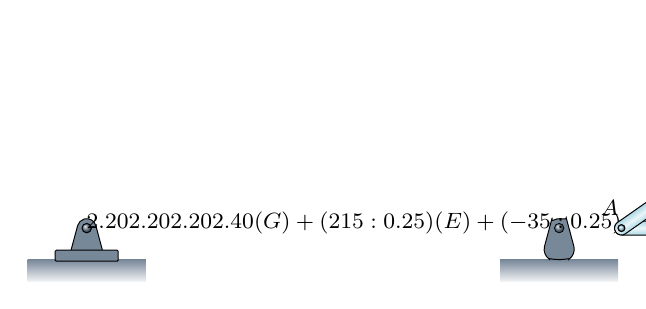
\begin{tikzpicture}

    % \def\offset{0.4}  

	\coordinate (A) at (0,0);
	\coordinate (B) at (2,0);
	\coordinate (C) at (4,0);
    \coordinate (D) at (6,0);
    \coordinate (F) at (3,2.1);
	\coordinate (E) at ($ (D)!0.4468!(F) $);	
    \coordinate (G) at ($ (A)!0.4468!(F) $); 
    
    \gettikzxy{(A)}{\ax}{\ay}
	\gettikzxy{(B)}{\bx}{\by}
	\gettikzxy{(C)}{\cx}{\cy}
	\gettikzxy{(D)}{\dx}{\dy}
	\gettikzxy{(E)}{\ex}{\ey}
	\gettikzxy{(F)}{\fx}{\fy}
    \gettikzxy{(G)}{\gx}{\gy}

	\shade[top color = LightSlateGray, bottom color = LightSlateGray!10] ($(A)+(-0.75,-0.4)$) rectangle +(1.5,-0.275);
    \shade[top color = LightSlateGray, bottom color = LightSlateGray!10] ($(D)+(-0.75,-0.4)$) rectangle +(1.5,-0.275);
    
    
    \Rocker{D}{LightSlateGray}{black}{0.4}{0.125}
    \PinnedConnection{A}{LightSlateGray}{black}{0.4}{0.125}
    
    \draw[thin, black] (\ax, \ay-0.175cm) -- ++(0,-1.125);
    \draw[thin, black] (\bx, \ay-0.175cm) -- ++(0,-1.125);
    \draw[thin, black] (\cx, \ay-0.175cm) -- ++(0,-1.125);
    \draw[thin, black] (\dx, \ay-0.175cm) -- ++(0,-1.125);
    \draw[thin, black] (\fx-0.35cm, \fy) -- (\ax-1cm,\fy);
    \draw[thin, black] (\ax-0.25cm, \ay) -- (\ax-1cm,\ay);

    \footnotesize
    \draw[Stealth-Stealth] (\ax, \ay-1cm) -- node[fill=white]{$2.20$ m}(\bx, \by-1cm);
    \draw[Stealth-Stealth] (\bx, \ay-1cm) -- node[fill=white]{$2.20$ m}(\cx, \by-1cm);
    \draw[Stealth-Stealth] (\cx, \ay-1cm) -- node[fill=white]{$2.20$ m}(\dx, \by-1cm);
    \draw[Stealth-Stealth] (\ax-0.625cm, \ay) -- node[fill=white]{$2.40$ m}(\ax-0.625cm, \fy);
    
    % \draw[thin] ($ (G)+(35:0.25) $) -- ++(-55:0.25)--++(215:0.25);
    \draw[thin] ($ (G)+(215:0.25) $) -- ++(305:0.25)--++(35:0.25);
    \draw[thin] ($ (E)+(-35:0.25) $) -- ++(-125:0.25)--++(145:0.25);
    % \draw[thin] ($ (E)+(145:0.25) $) -- ++(235:0.25)--++(325:0.25);

    \node[xshift=-4.75mm,yshift=2.5mm] at (B) {$\theta$};
    \node[xshift=3.5mm, yshift=2.5mm] at (B) {$\phi$};
    	
    \Member{C}{E}{LightBlue}{LightBlue!25}{black}{0.175}{0.0874}{0.125}
    \Member{B}{G}{LightBlue}{LightBlue!25}{black}{0.175}{0.0874}{0.125}
	\Member{A}{B}{LightBlue}{LightBlue!25}{black}{0.175}{0.0874}{0.125}
	\Member{B}{F}{LightBlue}{LightBlue!25}{black}{0.175}{0.0874}{0.125}
	\Member{C}{F}{LightBlue}{LightBlue!25}{black}{0.175}{0.0874}{0.125}
    \Member{C}{D}{LightBlue}{LightBlue!25}{black}{0.175}{0.0874}{0.125}
    \Member{D}{E}{LightBlue}{LightBlue!25}{black}{0.175}{0.0874}{0.125}
    \Member{E}{F}{LightBlue}{LightBlue!25}{black}{0.175}{0.0874}{0.125}
    \Member{A}{G}{LightBlue}{LightBlue!25}{black}{0.175}{0.0874}{0.125}
	\Member{G}{F}{LightBlue}{LightBlue!25}{black}{0.175}{0.0874}{0.125}
	\Member{B}{C}{LightBlue}{LightBlue!25}{black}{0.175}{0.0874}{0.125}
	
    \footnotesize
	\shadedraw[ball color=LightBlue] (A) circle (1.25pt) node[xshift=-1.5mm, yshift=2.5mm] {$A$};
	\shadedraw[ball color=LightBlue] (B) circle (1.25pt) node[xshift=2mm, yshift=-2.5mm] {$B$};
	\shadedraw[ball color=LightBlue] (C) circle (1.25pt) node[xshift=2mm, yshift=-2.5mm] {$C$};
	\shadedraw[ball color=LightBlue] (D) circle (1.25pt) node[xshift=1.5mm, yshift=2.5mm] {$D$};
	\shadedraw[ball color=LightBlue] (E) circle (1.25pt) node[xshift=1.5mm, yshift=2mm] {$E$};
	\shadedraw[ball color=LightBlue] (F) circle (1.25pt) node[yshift=2.5mm] {$F$};
    \shadedraw[ball color=LightBlue] (G) circle (1.25pt) node[xshift=-1.5mm, yshift=2mm] {$G$}; 
    
    

\end{tikzpicture}

  }
\end{frame}

%%%%%%%%%%%%%%%%%%%%%%%%%%%%%%%%%%%%%%%%%%%%%%%%%%%%%%%%%%%%%%%%%%%%%%%%%%%%%%%%%%%%%%%%%%%%%%%%%%%
\begin{frame}{pikz/01MathReview/math03}  
  % !TEX root = ../../statikz2020/statikz2020.tex

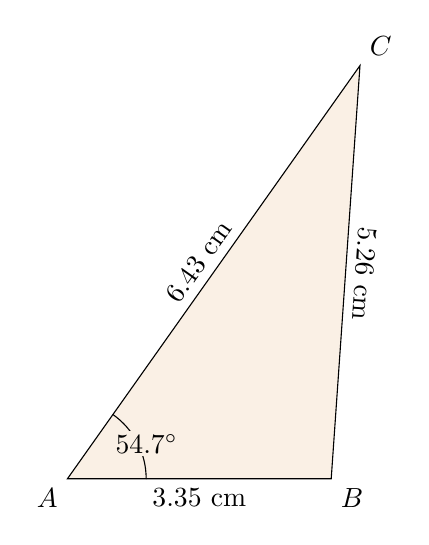
\begin{tikzpicture}[scale=\scale]

	\coordinate (A) at (0,0);
	\coordinate (B) at (3.35,0);
	\coordinate (C) at ($ (A) + (54.7:6.43) $);

	\filldraw[fill=Linen, draw=black] (A) -- node[sloped, above] {$6.43$ cm} (C) -- node[sloped, above, rotate=180]{$5.26$ cm}(B) -- node[below, sloped] {$3.35$ cm} cycle;
	% \node[above, rotated] at ($ (A)!0.5!(C)$) {$6.00$};


	\draw[below right] (B) node {$B$};
	\draw[below left] (A) node {$A$};
	\draw[above right] (C) node {$C$};

	\draw (1,0)  arc(0:54.7:1) node[fill=Linen, inner sep=0.4mm] at (24:1.1){$54.7^\circ$};



\end{tikzpicture}
 
\end{frame}

%%%%%%%%%%%%%%%%%%%%%%%%%%%%%%%%%%%%%%%%%%%%%%%%%%%%%%%%%%%%%%%%%%%%%%%%%%%%%%%%%%%%%%%%%%%%%%%%%%%
\begin{frame}{pikz/01MathReview/math04}
  \resizebox{0.5\textwidth}{!}{%
    % !TEX root = ../../statikz2020/statikz2020.tex

\makeatletter
\providecommand{\gettikzxy}[3]{%
	\tikz@scan@one@point\pgfutil@firstofone#1\relax
	\edef#2{\the\pgf@x}%
	\edef#3{\the\pgf@y}%
}
\makeatother


\begin{tikzpicture}[scale=\scale]

	\def\thickness{thick}
	% \def\stroke{black}
	\def\hi{.225}
	\def\radii{.225}
	\def\extend{0.225}

	\def\offset{0.4}

	\coordinate (E) at (0,0);
	\coordinate (F) at (3,0);
	\coordinate (G) at (6,0);
	\coordinate (A) at (9,0);
	\coordinate (B) at (6,2.5);
	\coordinate (C) at (3,3.75);
	\coordinate (D) at (0,5);
	\coordinate (Right) at ($ (A)+(1.5,0)$);
	\coordinate (Bottom) at ($ (A)+(0,-1.5)$);

	\shade[right color = DarkGrey, left color = LightGrey] ($(D)+(-0.66,1)$) rectangle ($(E)+(-2,-1.5)$);
	\draw[black] ($(D)+(-0.66,1)$) -- ($(E)+(-0.66,-1.5)$);

	\PinnedConnection[-90]{D}{DarkGrey}{black}{0.65}{0.125}
	\PinnedConnection[-90]{E}{DarkGrey}{black}{0.65}{0.125}


	\gettikzxy{(A)}{\ax}{\ay}
	\gettikzxy{(B)}{\bx}{\by}
	\gettikzxy{(C)}{\cx}{\cy}
	\gettikzxy{(D)}{\ddx}{\ddy}
	\gettikzxy{(E)}{\ex}{\ey}
	\gettikzxy{(F)}{\fx}{\fy}
	\gettikzxy{(G)}{\gx}{\gy}
	\gettikzxy{(Right)}{\rx}{\ry}
	\gettikzxy{(Bottom)}{\bbx}{\bby}

	\draw ($ (A)+(\offset,0)$) -- (\rx,\ay);
	\draw ($ (B)+(1.25*\offset,0)$) -- (\rx,\by);
	\draw ($ (C)+(2*\offset,0)$) -- (\rx,\cy);
	\draw ($ (D)+(2*\offset,0)$) -- (\rx,\ddy);
	\draw ($ (D)+(0, -\offset)$) -- (\ex,\ey+1.25*\offset cm);
	\draw ($ (E)+(0, -\offset)$) -- (\ex,\bby);
	\draw ($ (F)+(0, -\offset)$) -- (\fx,\bby);
	\draw ($ (G)+(0, -\offset)$) -- (\gx,\bby);
	\draw ($ (A)+(0, -\offset)$) -- (\ax,\bby);

	\Large
	\draw[latex-latex] (\ex,\bby+\offset cm) -- node[fill=white] {$3.00$ m}(\fx,\bby+\offset cm);
	\draw[latex-latex] (\fx,\bby+\offset cm) -- node[fill=white] {$3.00$ m}(\gx,\bby+\offset cm);
	\draw[latex-latex] (\gx,\bby+\offset cm) -- node[fill=white] {$3.00$ m}(\ax,\bby+\offset cm);
	\draw[latex-latex] (\rx-\offset cm,\ay) -- node[fill=white] {$2.50$ m}(\rx-\offset cm,\by);
	\draw[latex-latex] (\rx-\offset cm,\by) -- node[fill=white] {$1.25$ m}(\rx-\offset cm,\cy);
	\draw[latex-latex] (\rx-\offset cm,\cy) -- node[fill=white] {$1.25$ m}(\rx-\offset cm,\ddy);
	

	% \pgfoonew \BC=new rr(B,C,Burlywood1,black, 0.2)
	% \pgfoonew \CD=new rr(C,D,Burlywood1,black, 0.2)
	% \pgfoonew \EF=new rr(E,F,Burlywood1,black, 0.2)
	% \pgfoonew \FG=new rr(G,F,Burlywood1,black, 0.2)
	% \pgfoonew \AG=new rr(A,G,Burlywood1,black, 0.2)
	% \pgfoonew \AB=new rr(A,B,Burlywood1,black, 0.2)
	% \pgfoonew \CE=new rr(C,E,Burlywood1,black, 0.2)
	% \pgfoonew \BF=new rr(B,F,Burlywood1,black, 0.2)
	% \pgfoonew \CF=new rr(C,F,Burlywood1,black, 0.2)
	% \pgfoonew \BG=new rr(B,G,Burlywood1,black, 0.2)

	\Member{B}{C}{DarkKhaki}{DarkKhaki!25}{black}{0.35}{0.175}{.25}
    \Member{C}{D}{DarkKhaki}{DarkKhaki!25}{black}{0.35}{0.175}{.25}
    \Member{E}{F}{DarkKhaki}{DarkKhaki!25}{black}{0.35}{0.175}{.25}
    \Member{F}{G}{DarkKhaki}{DarkKhaki!25}{black}{0.35}{0.175}{.25}
    \Member{A}{G}{DarkKhaki}{DarkKhaki!25}{black}{0.35}{0.175}{.25}
    \Member{A}{B}{DarkKhaki}{DarkKhaki!25}{black}{0.35}{0.175}{.25}
	\Member{C}{E}{DarkKhaki}{DarkKhaki!25}{black}{0.35}{0.175}{.25}
	\Member{B}{F}{DarkKhaki}{DarkKhaki!25}{black}{0.35}{0.175}{.25}
    \Member{C}{F}{DarkKhaki}{DarkKhaki!25}{black}{0.35}{0.175}{.25}
    \Member{B}{G}{DarkKhaki}{DarkKhaki!25}{black}{0.35}{0.175}{.25}

	

	

	\shadedraw[ball color=Burlywood4] (A) circle (2.5pt) node[xshift=2mm, yshift=-3mm] {$A$};
	\shadedraw[ball color=Burlywood4] (B) circle (2.5pt) node[xshift=2.5mm, yshift=3.5mm] {$B$};
	\shadedraw[ball color=Burlywood4] (C) circle (2.5pt) node[xshift=2.5mm, yshift=3.5mm] {$C$};
	\shadedraw[ball color=Burlywood4] (D) circle (2.5pt) node[xshift=2.5mm, yshift=3.5mm] {$D$};
	\shadedraw[ball color=Burlywood4] (E) circle (2.5pt) node[xshift=2mm, yshift=-4mm] {$E$};
	\shadedraw[ball color=Burlywood4] (F) circle (2.5pt) node[xshift=2mm, yshift=-4mm] {$F$};
	\shadedraw[ball color=Burlywood4] (G) circle (2.5pt) node[xshift=2mm, yshift=-4mm] {$G$};



	% \draw[very thin,color=gray] (-0.3,-2.3) grid (2.9,3.3);
	% \draw[->] (-0.2,0) -- (3.2,0) node[right] {$x$};
	% \draw[->] (0,-2.5) -- (0,3.8) node[above] {$y$};
	% \draw[domain=-0.2:2.5, color=red, thick] plot[id=1] function{(7-2*x)/3}
	% node[below] {$2x+3y=7$};
	% \draw[domain=-0.2:0.8, color=blue, thick] plot[id=2] function{6*x-1}
	% node[right] {$6x-y=1$};

\end{tikzpicture}

  }
\end{frame}

%%%%%%%%%%%%%%%%%%%%%%%%%%%%%%%%%%%%%%%%%%%%%%%%%%%%%%%%%%%%%%%%%%%%%%%%%%%%%%%%%%%%%%%%%%%%%%%%%%%
\begin{frame}{pikz/01MathReview/math05}
  % !TEX root = ../../statikz2020/statikz2020.tex

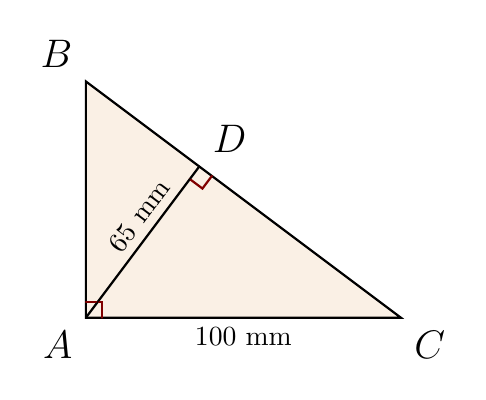
\begin{tikzpicture}

    \Large

	\coordinate (A) at (0,0);
	\coordinate (B) at (0,3);
	\coordinate (C) at (4,0);
	\coordinate (D) at ($(B)!0.36!(C)$);
	

    \gettikzxy{(A)}{\ax}{\ay}
    \gettikzxy{(B)}{\bx}{\by}
    \gettikzxy{(C)}{\cx}{\cy}
    \gettikzxy{(D)}{\dx}{\dy}
    
   \filldraw[fill=Linen, thick] (A)--(B)--(C)--cycle; 
   \draw[thick] (A)--(D); 
   \draw[Maroon, thick] (\ax+2mm,\ay)-- ++(0,0.2)-- ++(-0.2,0);
   \draw[Maroon, thick] ($(D)+(-36.9:0.2)$)-- ++(-126.9:0.2)-- ++(143.1:0.2);

   \node[below left] at (A){$A$};
   \node[above left] at (B){$B$};
   \node[below right] at (C){$C$};
   \node[above right] at (D){$D$};

   \normalsize

   \node[below] at ($(A)!0.5!(C)$){$100$ mm};
   \draw  (A) -- (D) node [sloped,pos=0.6,above] {$65$ mm};

\end{tikzpicture}

% \begin{tikzpicture}[domain=0:4]
% \draw[very thin,color=gray] (-0.1,-1.1) grid (3.9,3.9);
% \draw[->] (-0.2,0) -- (4.2,0) node[right] {$x$};
% \draw[->] (0,-1.2) -- (0,4.2) node[above] {$f(x)$};
% \draw[color=red] plot[id=x] function{x} node[right] {$f(x) =x$};
% \draw[color=blue] plot[id=sin] function{sin(x)} node[right] {$f(x) = \sin x$};
% \draw[color=orange] plot[id=exp] function{0.05*exp(x)} node[right] {$f(x) = \frac{1}{20} \mathrm e^x$};
% \end{tikzpicture}
\end{frame}

%%%%%%%%%%%%%%%%%%%%%%%%%%%%%%%%%%%%%%%%%%%%%%%%%%%%%%%%%%%%%%%%%%%%%%%%%%%%%%%%%%%%%%%%%%%%%%%%%%%
\begin{frame}{pikz/01MathReview/math06}
  % !TEX root = ../../statikz2020/statikz2020.tex

\begin{tikzpicture}

   

	\coordinate (O) at (0,0);
	\coordinate (A) at (0,-2);
	\coordinate (B) at (4,0);
	\coordinate (C) at (2,-3);	

    \gettikzxy{(A)}{\ax}{\ay}
    \gettikzxy{(B)}{\bx}{\by}
    \gettikzxy{(C)}{\cx}{\cy}
    \gettikzxy{(O)}{\ox}{\oy}

    \footnotesize
    \draw[thin] ($(C)+(-1,0)$)--($(C)+(0.65,0)$);
    \draw[thin, Green] (A)--node[above, sloped, black]{$1.350$ m}(C);
    \draw[thin, Green] (B)--node[above, sloped, black]{$2.90$ m}(C);
    \draw[thin, Green] (C)-- +(0,-1);
    \Member{A}{C}{DarkGreen}{DarkGreen!20}{black}{0.0625}{0.014}{0.0625};
    \Member{B}{C}{DarkGreen}{DarkGreen!20}{black}{0.0625}{0.014}{0.0625};
    \Member{C}{W}{DarkGreen}{DarkGreen!20}{black}{0.0625}{0.014}{0.0625};

    \small
    \fill[ball color=DarkGreen]  (A)circle(2pt)node[above right]{$A$};
    \fill[ball color=DarkGreen]  (B)circle(2pt)node[below right]{$B$};
    \fill[ball color=DarkGreen]  (C)circle(2pt)node[below right]{$C$};

    \fill[fill=DarkGoldenrod] ($(A)+(0,-3.5)$)--(O)--($(B)+(1,0)$)-- ++(0,1)--(\ox-1cm,\oy+1cm)--(\ox-1cm,\ay-3.5cm)--cycle;
    \draw ($(A)+(0,-3.5)$)--(O)--($(B)+(1,0)$);

    \node[xshift=-0.7cm,yshift=1.5mm] at (C) {$\theta$};
    \node[xshift=0.35cm,yshift=1.75mm] at (C) {$\phi$};

    \node[above left] at (O) {$O$};


    \shade[left color = SlateGray, right color = SlateGray, middle color = Silver!20] (\cx+0.35cm,\cy-1cm)-- ++(0.35,-1)-- ++(-1.4,0)-- ++(0.35,1)--cycle;
    \draw (\cx+0.35cm,\cy-1cm)-- ++(0.35,-1)-- ++(-1.4,0)-- ++(0.35,1)--cycle;

    \draw (\ax-2.5mm,\ay)--(\ax-7.5mm,\ay);
    \draw (\ox-2.5mm,\oy)--(\ox-7.5mm,\oy);
    \draw[Stealth-Stealth] (\ax-5mm,\ay)--node[fill=DarkGoldenrod, sloped]{$1.500$ m}(\ox-5mm,\oy);

    \draw (\ox,\oy+2.5mm)--(\ox,\oy+7.5mm);
    \draw (\bx,\by+2.5mm)--(\bx,\by+7.5mm);
    \draw[Stealth-Stealth] (\ox,\oy+5mm)--node[fill=DarkGoldenrod, sloped]{$3.00$ m}(\bx,\by+5mm);
    
    \node at ($(C)+(0,-1.5)$){\large $W$};


\end{tikzpicture}

\end{frame}

%%%%%%%%%%%%%%%%%%%%%%%%%%%%%%%%%%%%%%%%%%%%%%%%%%%%%%%%%%%%%%%%%%%%%%%%%%%%%%%%%%%%%%%%%%%%%%%%%%%
\section{Forces \& Components}

%%%%%%%%%%%%%%%%%%%%%%%%%%%%%%%%%%%%%%%%%%%%%%%%%%%%%%%%%%%%%%%%%%%%%%%%%%%%%%%%%%%%%%%%%%%%%%%%%%%

\section{Frames \& Machines}

\begin{frame}{Frames \& Machines}
  complex frames will start here

  \ifnum\pdfshellescape=1
 Yes, enabled
\else
 No, disabled
\fi
\end{frame}

\end{document}
